\chapter{Implementation}
\label{ch:implementation}

\emph{In this section, you should present what you have done. How things have been implemented and how they work.
Please avoid putting lines and lines of code here. But you can highlight some important elements of your implementations (some important part of the code, if necessary).}

\section{Structure of the Simulation}
\emph{Explain why you chose this structure and why you chose these hallucinations and sentences}

The structure of the simulation was carefully designed to evoke a progressively immersive and unsettling representation of hallucinations associated with schizophrenia. This structure was chosen to reflect both phenomenological research on psychotic symptoms and evidence-based educational strategies for increasing empathy and reducing stigma in health professionals.

The auditory hallucinations used in this simulation draw from documented simulation programs such as Patricia Deegan’s “Hearing Voices,” which have been shown to significantly impact empathy levels in students and clinicians \cite{Hsia2022}. In alignment with these findings, the simulation integrates a sequence of whispered voices and confrontational phrases. The sentences were crafted and timed intentionally to gradually escalate in emotional intensity, following research that demonstrates increased affective engagement leads to more powerful learning and emotional responses \cite{Skoy2016}.

Complementing the auditory component are visual hallucination elements, including dynamically spawning colored spheres, spatial distortions through dot placements, and visual darkening of the field of view. These visuals were inspired by clinical descriptions of visual hallucinations in psychotic disorders, such as geometric distortions, flickering lights, and anthropomorphic or symbolic figures \cite{Silverstein2021,Vanommen2019}.

The structural design aims to simulate both simple and complex hallucinations. Early stimuli (whispers, darkness) mimic the subtle onset of perceptual anomalies, while the crescendo of auditory cues and visual manifestations evoke the overwhelming nature of full-blown psychosis. This approach allows users to move from discomfort to disorientation, simulating the lived experience of progressive symptom development.

\section{Implementation of the Simulation}
\emph{Explain how you implemented the simulation. What are the main components of the simulation? How do they interact with each other?}
The simulation was implemented in Unity and constructed through modular components that interact in time-dependent sequences coordinated by a central control script.

\subsection{Orchestration}
At the heart of the system lies the \textit{Orchestrator.cs} script. This script sequences the entire simulation, controlling when sounds play, visual hallucinations appear, and environmental effects occur. The timeline was structured using IEnumerator coroutines, allowing asynchronous timed execution of events, ensuring immersive pacing without overwhelming the user too early in the experience.

Synchronization across components ensures the user is not overwhelmed with concurrent stimuli too early. For example, whispers begin before visuals, allowing users to acclimate to auditory disturbances before confronting the more jarring visual phenomena. Visual hallucinations are also paced in relation to emotional escalation in the voice samples, building tension across the timeline.

\begin{figure}[h!]
    \centering
    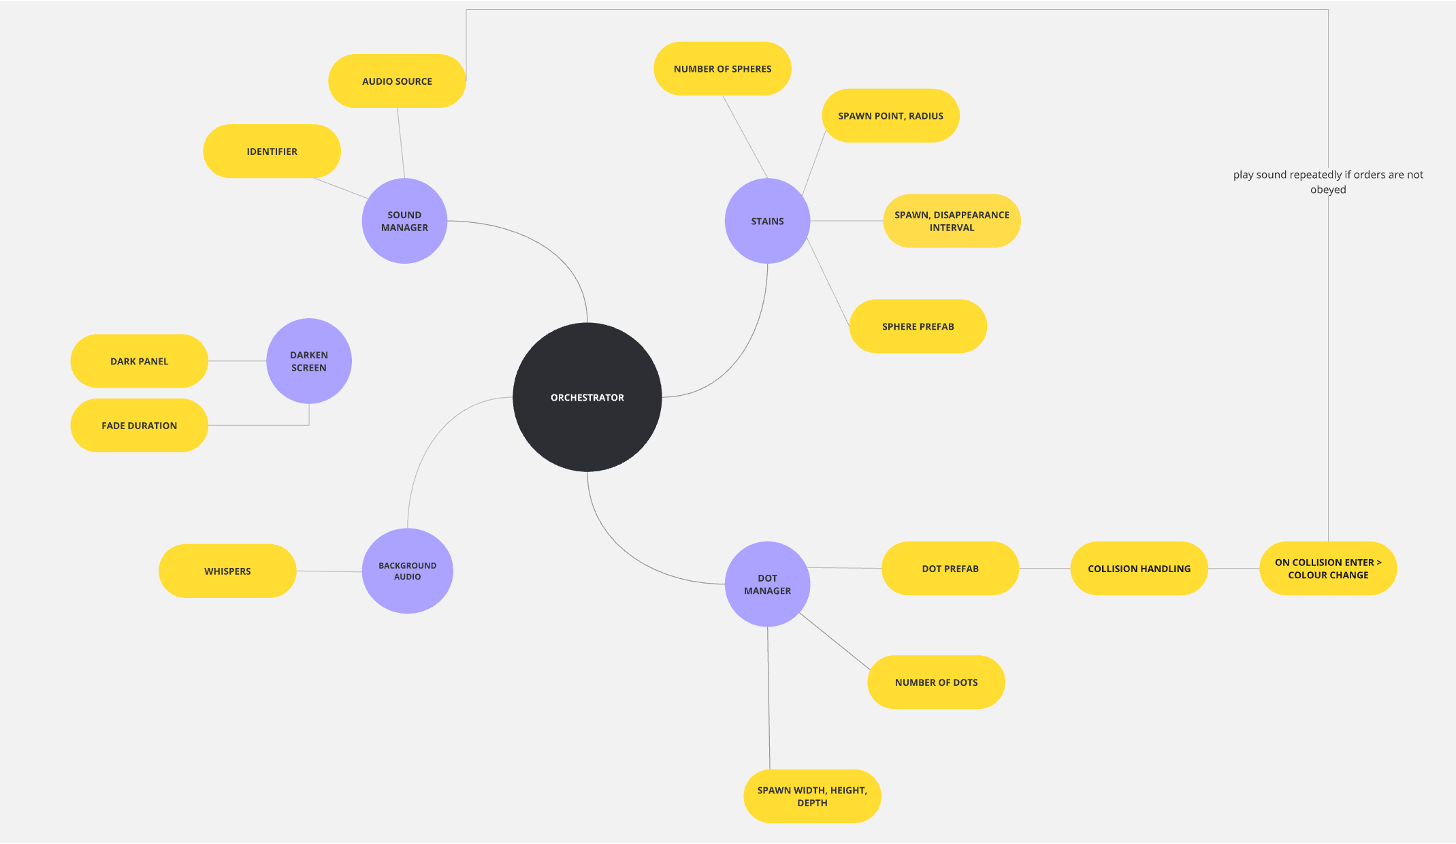
\includegraphics[width=0.8\textwidth]{../../Figures/Orch-sequence.png}
    \caption{Diagram of the Orchestrator system showing the interaction between auditory, visual, and environmental components.}
    \label{fig:orchestrator}
\end{figure}


\subsection{Auditory Hallucinations}

The auditory effects in the system are handled by the \textit{SoundManager.cs} script. Audio files are grouped by voice type, making it easy to play back different kinds of hallucination samples. These voices include phrases that sound accusatory, confusing, or frightening—reflecting common real-world descriptions of auditory hallucinations.
    
The voices were generated using ElevenLabs, a text-to-speech AI engine \cite{elevenlabs}. Each one was created with a specific emotional tone in mind: one voice sounds scared and almost shouting, another is snooty and mean, and the third sounds lost and desperate. These voices are played at key moments to create a stronger sense of fear, confusion, or paranoia. Their timing is matched with visual effects to create a more immersive and realistic experience of multisensory hallucinations.
    
In addition, the \textit{ObjectCollision.cs} script adds interactive audio that loops until the user physically interacts with an object. This mimics the frustrating and unpredictable nature of hallucinations, as often described by people experiencing psychosis.
    
    
\subsection{Visual Hallucinations}
Visual components are diversified to simulate various hallucination types:
\begin{itemize}
    \item Wave Deformation: \textit{DynamicWaveDeformation.cs} distorts object surfaces using transformations, creating a pulsating geometry that mimics perceptual distortions in psychosis.
    \item Gradual Screen Darkening: \textit{ScreenDarkener.cs} overlays a semi-transparent black UI panel to simulate the narrowing of visual perception or "tunnel vision," often reported during intense hallucinations.
    \item Dot Fields: \textit{DotManager.cs} creates random red and blue dots that appear above the user. These dots represent chaotic visual input or visual noise, similar to the floating patterns often described by people experiencing psychosis.
    \item Pulsating Spheres: The Orchestrator periodically spawns spherical objects, creating a feeling of presence and spatial invasion. Their randomness and impermanence reflect transient hallucinations and visual object anomalies.
\end{itemize}

Each visual element in the system was designed based on descriptions of how people with schizophrenia may experience their symptoms. These experiences are often grouped into simple, geometric, and complex visual types \cite{Silverstein2021,Vanommen2019}.

The way the system is built makes it easy to expand in the future.

\section{Challenges During Implementation} \emph{Discuss the main challenges encountered during the simulation development and how they were overcome. Highlight important coding aspects where appropriate.}

Despite careful planning, several significant challenges emerged during the development of the simulation:

\subsection{Audio Loop Management} Initially, each interactive sphere instantiated its own sound playback. This led to multiple overlapping sound loops, significantly breaking immersion and user experience. The problem arose because the audio logic was not centralized — each sphere's ObjectCollision component independently triggered audio playback upon spawning.

To solve this issue, a shared audio management system was developed, which is a static AudioSource and coroutine created within ObjectCollision.cs. This means that only one looped sound source exists, and it is globally stopped when a user interacts with any sphere.

A key logic excerpt illustrating this centralization is:

\begin{quote} \small \texttt{if (sharedAudioSource == null) { sharedAudioSource = ...; coroutineHost = this; repeatCoroutine = coroutineHost.StartCoroutine(RepeatAudio());}} \end{quote}

This ensures no duplicate sounds occur, even with multiple spheres present.

\subsection{Hand Interaction and Finger Identification} 
A second major challenge was accurately detecting when a user touched a sphere. Initially, an additional \textit{poke interaction} module was mistakenly integrated alongside Unity's built-in collision detection. This redundant system caused conflicting behavior and unpredictable touch responses. Upon deeper inspection, it was discovered that Unity’s hand collision system already assigns specific identifiers to each fingertip collider, such as \textit{HandIndex1} for the index finger. Reliable detection could therefore be implemented simply by checking the collision object's name during a collision event, rather than adding redundant interaction modules.

\begin{quote} \small \texttt{if (collision.gameObject.name.Contains("HandIndex1")) { ... }} \end{quote}

By removing unnecessary modules and using direct collision name checks, touch interactions became smooth and predictable, immediately changing the spheres color and stopping the looping sound.

\subsection{Hardware-Related Sound Privacy} During preliminary testing, the built-in speakers of the Meta Quest 3 were found to be too loud, leaking audio to the entire room and affecting non-participant observers. To address this, PhoneLook bone-conduction headphones were integrated into the simulation setup. This had the advantage that the audio is transmitted privately to the participant without occluding ambient sounds.
It also ensures immersive simulatin while respecting privacy and the testing environment.

\subsection{Spatial Placement of Sound Sources} Another significant challenge was the spatial arrangement of audio sources within the 3D simulation environment. Initially, it was difficult to orient myself correctly in Unityss Scene View, making it unclear where the sounds would originate from relative to the user's position. Proper placement was essential to create a convincing spatial auditory experience, because sounds had to feel anchored in specific locations in the environment. As the user moved, the sounds needed to remain fixed in space, enhancing realism and immersion.

To solve this, I invested time to become familiar with Unity's camera controls and 3D scene navigation.Then, the sound sources were distributed strategically across different coordinates, ensuring that different hallucinated voices would come from distinct spatial directions.

An example of the 3D placement of the sound sources in the Unity scene is shown in \autoref{fig:sound_sources}.

\begin{figure}[h!] \centering 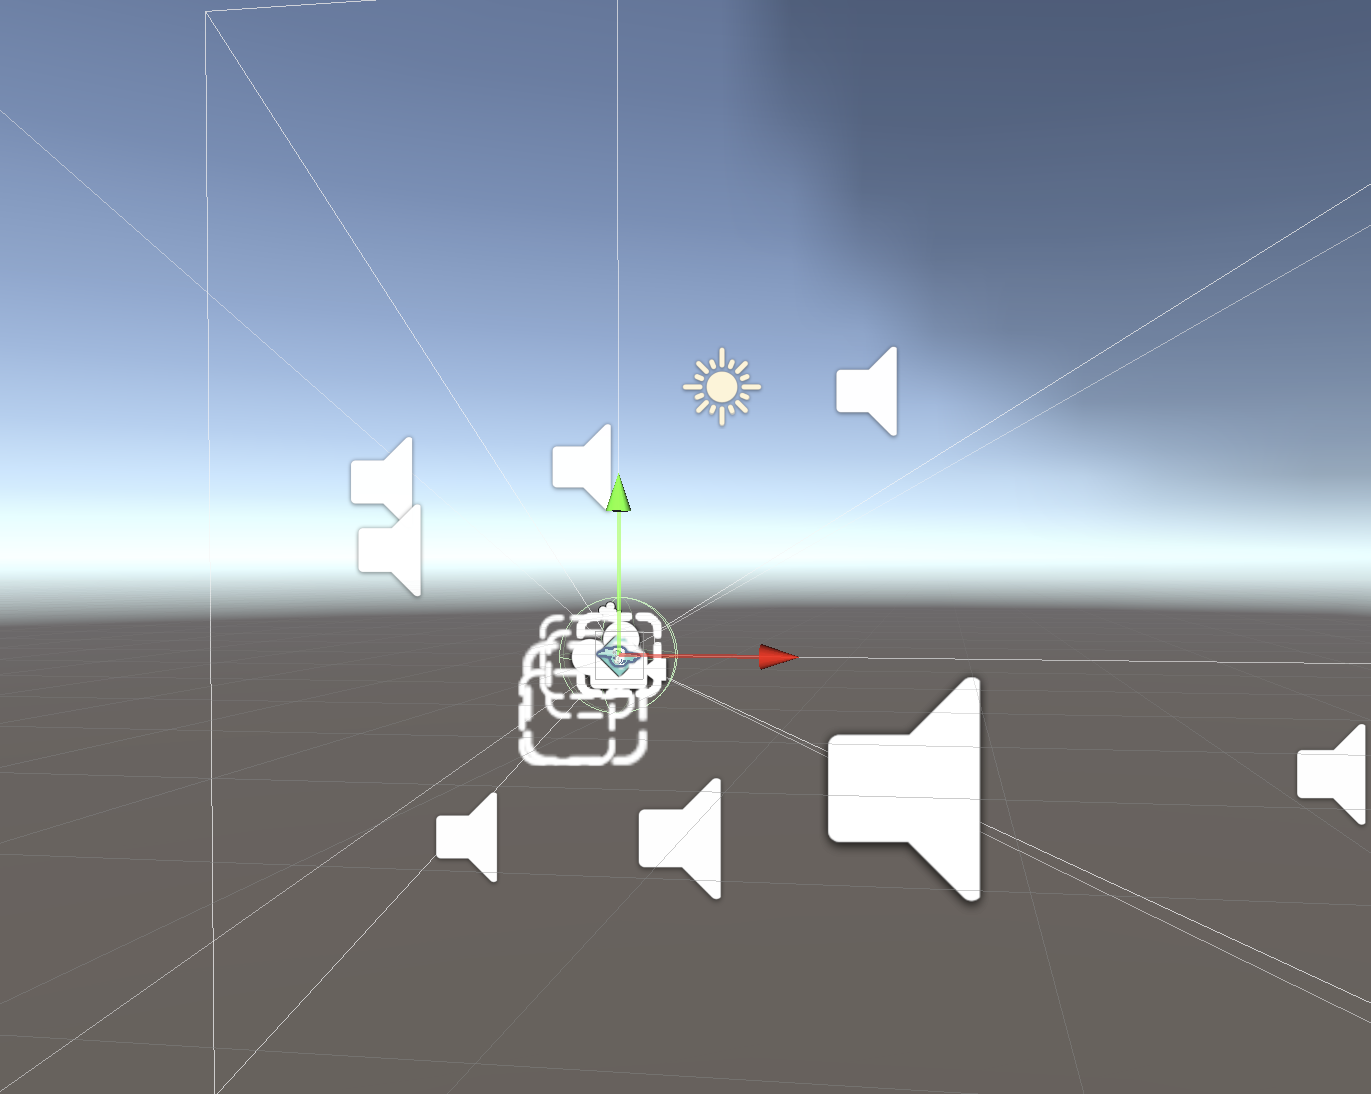
\includegraphics[width=0.8\textwidth]{../../Figures/unity-scene.png} \caption{Placement of spatial sound sources in the Unity scene for the hallucination simulation. Each speaker icon represents a sound source emitting a hallucination voice.} \label{fig:sound_sources} \end{figure}

